% !TeX root = ../tfg.tex
% !TeX encoding = utf8

\chapter{Descenso de Gradiente en un Problema OLS}\label{ap:apendiceC}

En este anexo se investiga el comportamiento del descenso de gradiente al aplicarse a un problema OLS, en comparación con la solución obtenida mediante la pseudoinversa.

El objetivo es encontrar la solución al mismo problema de regresión descrito en el apartado~\ref{subsubsec:funcion-lineal}, utilizando el descenso de gradiente y el error cuadrático medio como función de pérdida a minimizar, tanto para la base de Legendre como para la base polinomial clásica (omitiéndose la base redundante, al esperarse resultados similares a la base clásica). 

Para los valores de los hiperparámetros, se utiliza una tasa de aprendizaje de $10^{-2}$ y un número de épocas igual a $10000$.

\begin{figure}[h]
    \centering
    \begin{subfigure}[b]{0.48\textwidth}
        \centering
        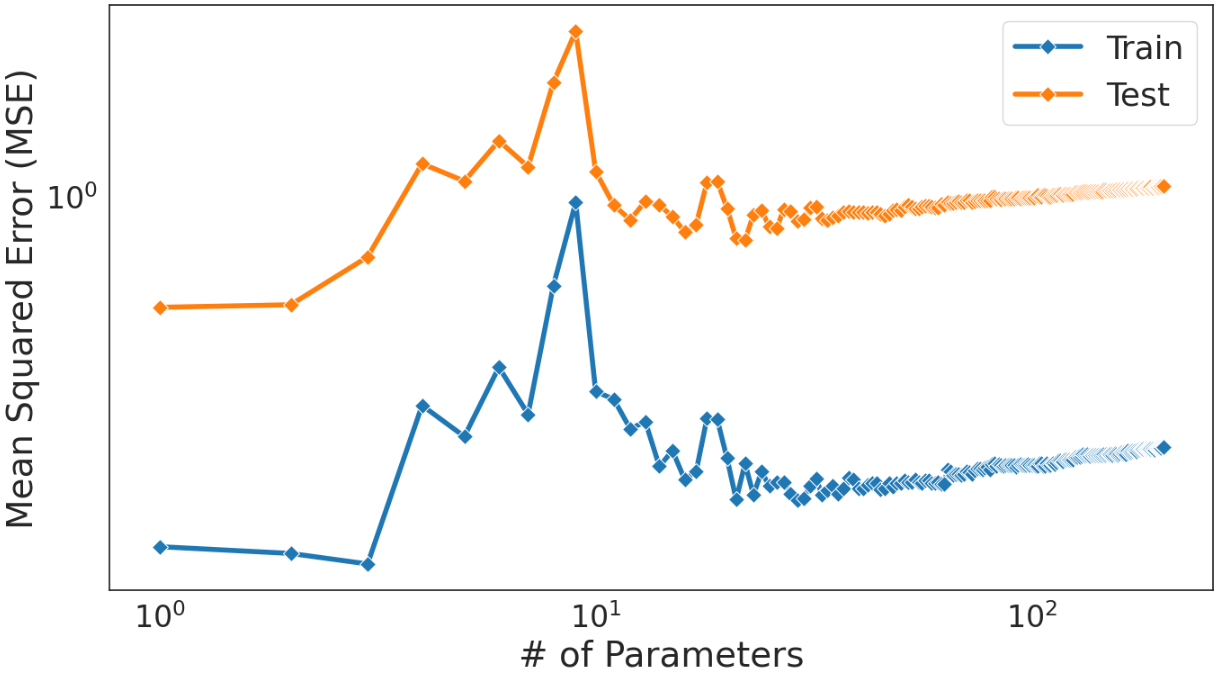
\includegraphics[width=\textwidth]{img/experiments/LegendreFeaturesGD_DDD.png}
        \caption{Aproximación de Legendre, donde se observa cómo se manifiesta el doble descenso.}\label{fig:LegendreFeaturesGD_DDD}
    \end{subfigure}
    \hfill
    \begin{subfigure}[b]{0.48\textwidth}
        \centering
        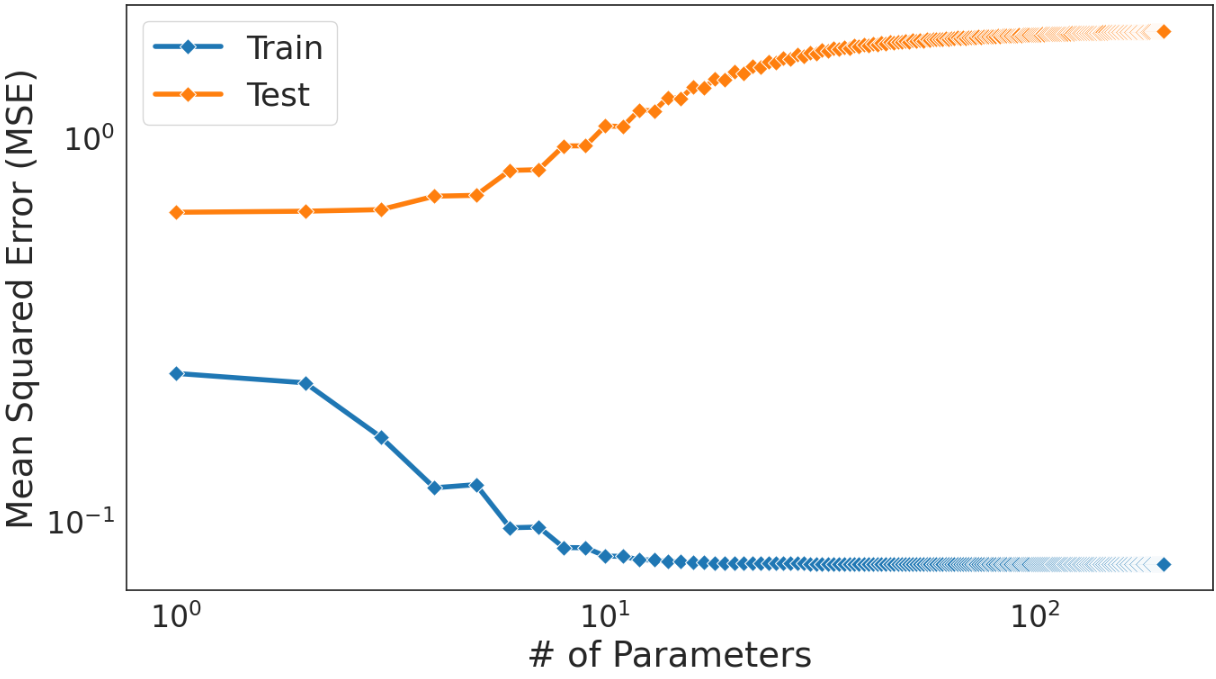
\includegraphics[width=\textwidth]{img/experiments/PolyFeaturesGD_DDD.png}
        \caption{Aproximación clásica, donde se observa cómo no se manifiesta el doble descenso.}\label{fig:PolyFeaturesGD_DDD}
    \end{subfigure}
    \caption[Error en entrenamiento y test para las aproximaciones de Legendre y clásica utilizando el GD.]{Error en entrenamiento y test para las aproximaciones de Legendre y clásica utilizando el GD.}\label{fig:aproximaciones-gd}
\end{figure}

La Figura~\ref{fig:aproximaciones-gd} muestra que los resultados obtenidos al utilizar el GD son similares a los obtenidos mediante la pseudoinversa (véase el apartado~\ref{subsubsec:funcion-lineal}, donde se manifiesta el doble descenso para la base de Legendre y no para la base polinomial clásica), con la salvedad de que el error de entrenamiento es mayor al emplear GD y no llega a ser nulo, aunque es bastante cercano.. Esto se debe a que, en el caso del GD, no estamos resolviendo de manera exacta una ecuación, sino que simplemente estamos aproximando la solución mediante un proceso iterativo, el cual requiere más tiempo para alcanzar un valor muy cercano a cero.

Como conclusión, se evidencia que, al emplear un gran tamaño de \textit{batch} y suficiente tiempo de entrenamiento (número de épocas), el descenso de gradiente tiende a aproximarse hacia la solución analítica que ofrece la pseudoinversa, tal y como se ha detallado (bajo ciertas condiciones) en la Subsección~\ref{subsec:problema-regresion}, y como también se expone en el trabajo de Lee et al.~\cite{Lee2016}.

\endinput
%------------------------------------------------------------------------------------
% FIN DEL APÉNDICE. 
%------------------------------------------------------------------------------------
